
\let\negmedspace\undefined
\let\negthickspace\undefined
\documentclass[journal]{IEEEtran}
\usepackage[a5paper, margin=10mm, onecolumn]{geometry}
%\usepackage{lmodern} % Ensure lmodern is loaded for pdflatex
\usepackage{tfrupee} % Include tfrupee package

\setlength{\headheight}{1cm} % Set the height of the header box
\setlength{\headsep}{0mm}     % Set the distance between the header box and the top of the text

\usepackage{gvv-book}
\usepackage{gvv}
\usepackage{cite}
\usepackage{amsmath,amssymb,amsfonts,amsthm}
\usepackage{amsmath}
\usepackage{algorithmic}
\usepackage{graphicx}
\usepackage{textcomp}
\usepackage{xcolor}
\usepackage{txfonts}
\usepackage{listings}
\usepackage{enumitem}
\usepackage{mathtools}
\usepackage{gensymb}
\usepackage{comment}
\usepackage[breaklinks=true]{hyperref}
\usepackage{tkz-euclide} 
\usepackage{listings}
% \usepackage{gvv}                                        
\def\inputGnumericTable{}                                 
\usepackage[latin1]{inputenc}                                
\usepackage{color}                                            
\usepackage{array}                                            
\usepackage{longtable}                                       
\usepackage{calc}                                             
\usepackage{multirow}                                         
\usepackage{hhline}                                           
\usepackage{ifthen}                                           
\usepackage{lscape}
\usepackage{circuitikz}
\tikzstyle{block} = [rectangle, draw, fill=blue!20, 
    text width=4em, text centered, rounded corners, minimum height=3em]
\tikzstyle{sum} = [draw, fill=blue!10, circle, minimum size=1cm, node distance=1.5cm]
\tikzstyle{input} = [coordinate]
\tikzstyle{output} = [coordinate]


\begin{document}

\bibliographystyle{IEEEtran}
\vspace{3cm}

\title{7.2.12}
\author{AI25BTECH11018-Hemanth Reddy}
 \maketitle
% \newpage
% \bigskip
{\let\newpage\relax\maketitle}

\renewcommand{\thefigure}{\theenumi}
\renewcommand{\thetable}{\theenumi}
\setlength{\intextsep}{10pt} % Space between text and floats


\numberwithin{equation}{enumi}
\numberwithin{figure}{enumi}
\renewcommand{\thetable}{\theenumi}

\textbf{Question:}\\

If the lines 2x - 3y = 5 and 3x - 4y = 7 are the diameters of a circle of area 154
square units, then obtain the equation of the circle.\\
\textbf{Solution:}\\

Let :
\begin{align}
    \vec{r_1} = \myvec{2 & -3 }\vec{k} = 5 \\
    \vec{r_2} = \myvec{3 & -4}\vec{k} = 7
\end{align}

The augmented matrix of the above equations is given by,\\
\begin{align}
    \myvec{ 2&-3&&5\\ 3&-4&&7} \stackrel{R_2 \leftarrow 2R_2 - 3R_1}{\longleftrightarrow}\myvec{ 2&-3&&5\\ 0&1&&-1} 
\end{align}

\begin{align}
    \myvec{2&-3&&5\\ 0&1&&-1} \stackrel{R_1 \leftarrow R_1 +3R_2}{\longleftrightarrow}\myvec{ 2&0&&2\\ 0&1&&-1} 
\end{align}

\begin{align}
    2x=2 \qquad x=1\\
    y=-1 
\end{align}

Point of intersection of diameters of circle is the center of circle $\vec{k}=\myvec{1\\-1}$\\
Given\\
\begin{center}
    Area of circle = $\pi r^2$ = 154 sq. units\\Using $\pi=\frac{22}{7}$  \qquad r=7 units\\
\end{center}

\begin{align}
    \text{Equation of circle is }||\vec{x}||^2 + 2\vec{u}^{\text{T}}\vec{x} + f = 0
\end{align}
\begin{align}
    \vec{u}=-\vec{k} \qquad f =||\vec{u}||^2 - r^2 
\end{align}

\begin{align}
    \vec{u}=\myvec{-1\\1} \qquad f=(\sqrt{2})^2 - 7^2 = -47\\
     \text{Equation of circle is }||\vec{x}||^2 + 2\myvec{-1&1}\vec{x} -47 = 0
\end{align}


\begin{figure}[H]
    \centering
    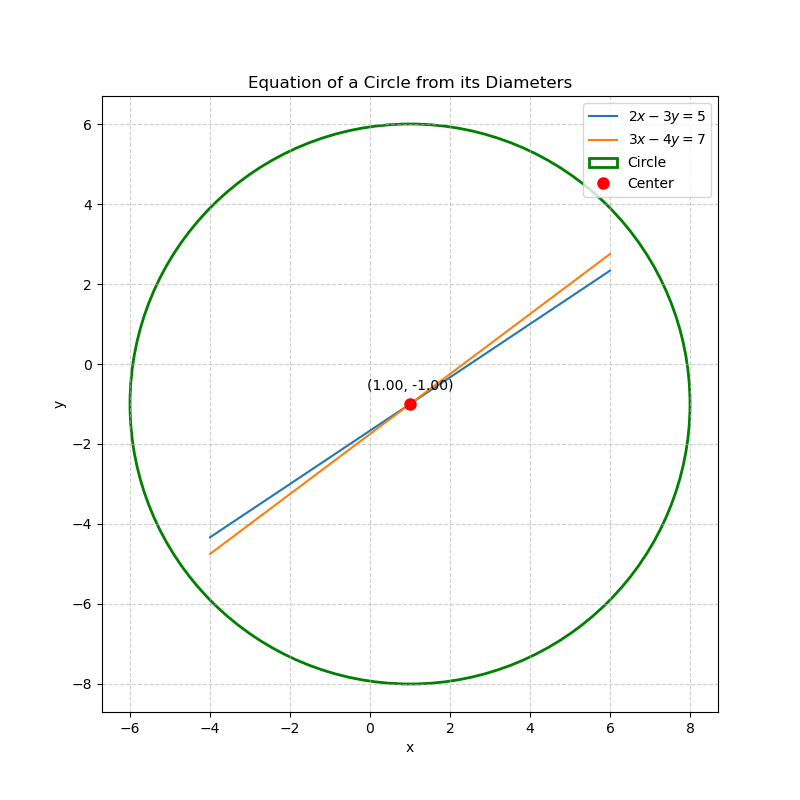
\includegraphics[width=0.8\linewidth]{figs/circle.png}
    \caption{}
    \label{fig:placeholder}
\end{figure}
\end{document}






